\documentclass[sigconf]{acmart}
\usepackage{amsmath, amsthm}
\usepackage{graphicx}
\usepackage{url}
\usepackage{hyperref}
\usepackage{booktabs}    % For better tables
\usepackage{xcolor}      % For colored text if needed
\usepackage{caption}     % For better control of captions
\usepackage{multirow}    % For multi-row table cells

\newtheorem{theorem}{Theorem}
\newtheorem{lemma}[theorem]{Lemma}
\newtheorem{proposition}[theorem]{Proposition}
\newtheorem{corollary}[theorem]{Corollary}
\newtheorem{definition}{Definition}
\newtheorem{remark}{Remark}

\AtBeginDocument{%
  \providecommand\BibTeX{{%
    Bib\TeX}}}

\setcopyright{acmlicensed}
\copyrightyear{2026}
\acmYear{2026}
\acmDOI{XXXXXXX.XXXXXXX}
\acmConference[SIGIR '26]{ACM SIGIR}{July 2026}{Washington D.C., USA}
\acmISBN{978-1-4503-XXXX-X/2026/07}



\title{Estimating Position Bias with Reduced Variance without Intrusive Interventions}

% \author{Alessandro Magnani}
% \email{almagnan@coupang.com}
% \affiliation{%
%   \institution{Coupang Inc.}
% }

% \author{Min Xie}
% \email{mixie@coupang.com}
% \affiliation{%
%   \institution{Coupang Inc.}
% }

% \renewcommand{\shortauthors}{Magnani et al.}

\author{Anonymous}
\affiliation{%
  \institution{Anonymous}
  \country{}}
\renewcommand{\shortauthors}{Anonymous}


\begin{document}

\begin{abstract}
Presentation bias remains a major challenge in learning-to-rank from implicit feedback, as it obscures the true relevance signal. Building upon intervention harvesting \cite{agarwal2019estimating}, which estimates position bias without intrusive randomization, we propose harmonic weighting—a novel weighting scheme for the ratio estimator that retains unbiasedness while significantly reducing variance. We establish an exact Cauchy–Schwarz guarantee that harmonic always reduces the delta-method variance surrogate $V_k+V_{k'}$, prove that harmonic weighting is variance-optimal in the symmetric setting ($\alpha=\beta$), and characterize when variance reduction extends to the asymmetric case via a decomposition theorem. Empirically, we demonstrate variance reductions of up to 55\% on synthetic imbalanced data, confirmed on semi-synthetic data using real relevance labels from the Yahoo LTR dataset. Lower variance translates directly to data efficiency: harmonic achieves the same estimation accuracy as the original estimator with roughly \textbf{half the data}. We also show that all unbiased methods share the same bias under Position-Based Model violations, making lower-variance estimation directly advantageous for mean squared error.
\end{abstract}

\maketitle

\section{Introduction}
\label{sec:introduction}

Position bias—where higher-ranked results receive disproportionate user attention—systematically corrupts click signals used for learning-to-rank \cite{joachims2017unbiased}. For instance, in e-commerce platforms a product at position~1 may receive 5--10$\times$ more clicks than an equally relevant item at position~10, creating a feedback loop that perpetuates suboptimal rankings. Unbiased learning requires accurate propensity estimates, but traditional approaches rely on costly randomized interventions (swap experiments, result randomization) that degrade user experience and cause revenue loss in production systems \cite{joachims2017unbiased, wang2018position}.

Recent advances in counterfactual learning-to-rank have shown that unbiased learning is possible when examination propensities are known \cite{joachims2017unbiased}. Estimating these propensities accurately remains challenging: traditional approaches rely on explicit randomized interventions that degrade user experience \cite{wang2018position}.

Intervention harvesting \cite{agarwal2019estimating} avoids explicit randomization by leveraging naturally occurring ranking variations across concurrently deployed rankers. However, the conventional weighting scheme produces high estimator variance when impression counts are imbalanced—a common situation in production A/B-testing environments where some documents accumulate disproportionate traffic at one position.

We propose harmonic weighting, a modified weighting scheme that addresses this critical limitation while retaining unbiasedness. Key contributions: (1) any count-dependent weight preserves ratio-unbiasedness; (2) an exact Cauchy–Schwarz guarantee that harmonic always reduces the variance surrogate $V_k + V_{k'}$, which implies lower $\mathrm{Var}(\hat{R})$ via the delta method; (3) exact optimality when propensities are equal; (4) up to 55\% variance reduction in synthetic and semi-synthetic (Yahoo LTR) experiments; (5) harmonic requires roughly \textbf{half the data} to match the original estimator's accuracy.

\section{Background and Preliminaries}
\label{sec:background}

\subsection{Position-Based Propensity Model (PBM)}
The Position-Based Model recognizes that higher-ranked results are more likely to be examined by users than lower-ranked results. For a query $q$ where document $d$ is displayed at position $k$, let $C$ be the random variable indicating whether the user clicks on $d$, and $E$ be the random variable denoting whether the user examines position $k$.

Following \cite{agarwal2019estimating}, we denote the relevance of a document as a non-random function $\textrm{rel}(q,d)$ of $q$, where $\textrm{rel}(q,d) = 1$ indicates relevant and $\textrm{rel}(q,d) = 0$ indicates non-relevant. According to the PBM \cite{richardson2007predicting, chuklin2015click}, the probability of a click is:

\begin{equation}
\mathrm{Pr}(C = 1|q,d,k) = \mathrm{Pr}(E = 1|k) \cdot \textrm{rel}(q,d) = p_k \cdot \textrm{rel}(q,d)
\end{equation}

where $p_k := \mathrm{Pr}(E = 1|k)$ is the examination probability, which depends only on the position $k$.


\subsection{Interventional Sets}
\label{sec:intervention-harvesting}

For each pair of positions $k \neq k' \in [M]$ (where $M$ is the number of positions of interest), \cite{agarwal2019estimating} defined interventional sets:
\begin{align*}
S_{k,k'} := \{(q,d) :\ & q \in Q, d \in \Omega(q),\\
& \exists f,f' \textrm{ s.t. } \textrm{rk}(d|f(q))=k,\\
& \textrm{rk}(d|f'(q))=k'\}
\end{align*}

Each interventional set $S_{k,k'}$ contains query-document pairs where the document appeared at position $k$ in one ranking and position $k'$ in another.

For each $(q,d) \in S_{k,k'}$, let $N_k^i$ and $N_{k'}^i$ denote the total impression counts at positions $k$ and $k'$ respectively, and let $C_k^i$, $C_{k'}^i$ denote the total click counts at each position.

\subsection{Ratio Estimator}
\label{sec:ratio-estimator}

For each interventional set $S_{k,k'}$, we consider a general weighted ratio estimator:
\begin{equation}
\hat{R}_{k,k'} = \frac{A}{B} = \frac{\sum_i \omega_i \cdot C_k^i / N_k^i}{\sum_i \omega_i \cdot C_{k'}^i / N_{k'}^i}
\end{equation}
where $\omega_i \geq 0$ are non-negative weights that may depend on the observation counts $N_k^i$, $N_{k'}^i$ but not on the click counts. Different choices of $\omega_i$ yield different weighting schemes. The original estimator of \cite{agarwal2019estimating} uses $\omega_i = N_k^i$. Under the ratio form in Eq.~(1), this is equivalently represented by constant pair weights $\omega_i = 1$: the $N_k^i$ factors in numerator and denominator cancel, leaving the same estimator. We present a unified framework for analyzing and improving upon this choice.

\section{Harmonic Weighting}
\label{sec:harmonic_weight}

\subsection{Weighting Schemes}

We consider the following weighting schemes, all of which use weights $\omega_i$ depending only on the observation counts:

\begin{itemize}
\item \textbf{Original}: $\omega_i = 1$ (constant; equivalent to \cite{agarwal2019estimating} as explained in Section~\ref{sec:ratio-estimator})
\item \textbf{Min-weighting}: $\omega_i = \min(N_k^i, N_{k'}^i)$
\item \textbf{Harmonic weighting} (our proposal):
\begin{equation}
\omega_i^h = \frac{N_k^i \cdot N_{k'}^i}{N_k^i + N_{k'}^i}
\end{equation}
\end{itemize}

The harmonic weight $\omega_i^h$ is the harmonic mean of $N_k^i$ and $N_{k'}^i$ up to a factor of $1/2$. It balances the contribution of each document pair by downweighting pairs with extreme impression imbalances.

We also compare against \textbf{clipped weighting} (subsampling the majority position when $N_k^i/N_{k'}^i > \tau$) \cite{bottou2013counterfactual}, which breaks ratio-unbiasedness and serves as a biased lower-variance reference.

\subsection{Ratio-Unbiasedness}

The following theorem shows that any weight function depending only on observation counts preserves the ratio-unbiasedness property.

\begin{theorem}[Ratio-unbiasedness]
\label{thm:ratio_unbiased}
Under the Position-Based Model, for any weights $\omega_i = \omega(N_k^i, N_{k'}^i) \geq 0$ that depend only on the observation counts (not on clicks), the ratio estimator satisfies:
\[
\frac{\mathbb{E}[A]}{\mathbb{E}[B]} = \frac{p_k}{p_{k'}}
\]
provided $\mathbb{E}[B] \neq 0$.
\end{theorem}

\begin{proof}
Since $\omega_i$ is independent of $C_k^i$ given $N_k^i, N_{k'}^i$, conditioning on counts:
\begin{align*}
\mathbb{E}[A] &= \mathbb{E}\left[\sum_i \omega_i \frac{C_k^i}{N_k^i}\right] = \sum_{(q,d)} \mathbb{E}\left[\omega_i \cdot \frac{\mathbb{E}[C_k^i | N_k^i, N_{k'}^i]}{N_k^i}\right]
\end{align*}

Under PBM, $\mathbb{E}[C_k^i | N_k^i, N_{k'}^i] = N_k^i \cdot p_k \cdot \textrm{rel}(q,d)$, so the $N_k^i$ terms cancel:
\begin{align*}
\mathbb{E}[A] &= p_k \sum_{(q,d)} \textrm{rel}(q,d) \cdot \mathbb{E}[\omega_i]
\end{align*}

By the same argument, $\mathbb{E}[B] = p_{k'} \sum_{(q,d)} \textrm{rel}(q,d) \cdot \mathbb{E}[\omega_i]$.

Taking the ratio and canceling the common factor (which is positive) yields $\mathbb{E}[A]/\mathbb{E}[B] = p_k/p_{k'}$.
\end{proof}

This theorem applies to original, min, and harmonic weighting. Clipped weighting violates this condition as it makes $\omega_i$ implicitly depend on which position has larger counts, breaking the symmetry required for unbiasedness.

\section{Variance Reduction Analysis}
\label{sec:variance_reduction}

\subsection{Delta-Method Variance}

We analyze the conditional variance of $\hat{R}_{k,k'} = A/B$ given observation counts $\mathbf{N}$. Since $A$ and $B$ are sums of independent terms (across documents), the delta method gives:

\begin{proposition}[Delta-method variance]
\label{prop:delta_method}
Conditionally on observation counts $\mathbf{N} = \{N_k^i, N_{k'}^i\}$:
\begin{equation}
\mathrm{Var}(\hat{R}_{k,k'} \mid \mathbf{N}) \approx R^2 \left[\alpha \cdot V_k(\omega) + \beta \cdot V_{k'}(\omega)\right]
\end{equation}
where $R = p_k/p_{k'}$, $\alpha = (1-p_k)/p_k$, $\beta = (1-p_{k'})/p_{k'}$, and:
\begin{equation}
V_r(\omega) = \frac{\sum_i \omega_i^2 / N_r^i}{\left(\sum_i \omega_i\right)^2}
\end{equation}
\end{proposition}

The terms $\alpha$ and $\beta$ capture the binomial variance at positions $k$ and $k'$ respectively. Since $p_k$ is typically larger for higher positions (higher examination probability), $\alpha$ tends to be smaller for positions closer to the top.

\noindent\textit{Note on proof structure.} The two theorems below are \textbf{exact} results for the variance surrogate $V_r(\omega)$; their implication for the actual ratio variance $\mathrm{Var}(\hat{R}\mid\mathbf{N})$ follows via the delta-method approximation above.

\subsection{Cauchy–Schwarz Guarantee}

Let $D_r = V_r(\omega^h) - V_r(1)$ denote the change in variance term at position $r$ when switching from original to harmonic weighting.

\begin{theorem}[Cauchy–Schwarz guarantee]
\label{thm:cs}
For any observation counts $\{N_k^i, N_{k'}^i\}_{i=1}^n$:
\[
D_k + D_{k'} \leq 0
\]
That is, harmonic weighting always reduces the sum of per-position variance terms compared to original weighting.
\end{theorem}

\begin{proof}
By direct computation:
\[
V_r(\omega^h) = \frac{\sum_i (\omega_i^h)^2 / N_r^i}{(\sum_i \omega_i^h)^2}, \quad V_r(1) = \frac{\sum_i 1/N_r^i}{n^2}
\]

The sum $V_k(\omega^h) + V_{k'}(\omega^h)$ can be written as:
\[
V_k + V_{k'} = \frac{\sum_i (\omega_i^h)^2 (1/N_k^i + 1/N_{k'}^i)}{W^2}
\]
where $W = \sum_i \omega_i^h$ and we used $\omega_i^h = \omega^h_i$ for both positions. Substituting $\omega_i^h = N_k^i N_{k'}^i / (N_k^i + N_{k'}^i)$, and noting that $(\omega_i^h)^2 (1/N_k^i + 1/N_{k'}^i) = (\omega_i^h)^2 \cdot (N_k^i + N_{k'}^i)/(N_k^i N_{k'}^i) = \omega_i^h$:
\[
V_k(\omega^h) + V_{k'}(\omega^h) = \frac{\sum_i \omega_i^h}{(\sum_i \omega_i^h)^2} = \frac{1}{\sum_i \omega_i^h} = \frac{1}{W}
\]

For the original estimator with $\omega_i = 1$:
\[
V_k(1) + V_{k'}(1) = \frac{1}{n^2}\sum_i \left(\frac{1}{N_k^i} + \frac{1}{N_{k'}^i}\right) = \frac{1}{n^2}\sum_i \frac{N_k^i + N_{k'}^i}{N_k^i N_{k'}^i} = \frac{1}{n^2}\sum_i \frac{1}{\omega_i^h}
\]

Since $W = \sum_i \omega_i^h$ and $\sum_i 1/\omega_i^h$, by the Cauchy–Schwarz inequality:
\[
n^2 \leq \left(\sum_i \omega_i^h\right)\left(\sum_i \frac{1}{\omega_i^h}\right) = W \cdot \sum_i \frac{1}{\omega_i^h}
\]

Therefore $1/W \leq (1/n^2)\sum_i 1/\omega_i^h$, i.e., $V_k(\omega^h) + V_{k'}(\omega^h) \leq V_k(1) + V_{k'}(1)$, which gives $D_k + D_{k'} \leq 0$.
\end{proof}

\begin{remark}
Theorem~\ref{thm:cs} is an exact, unconditional guarantee on the variance surrogate $V_k(\omega)+V_{k'}(\omega)$, holding for any impression counts. Via the delta-method approximation in Proposition~\ref{prop:delta_method}, this translates to a reduction in $\mathrm{Var}(\hat{R}\mid\mathbf{N})$ when $\alpha\approx\beta$ (Theorem~\ref{thm:optimality}) and more generally as established by Theorem~\ref{thm:decomp}. The bound is tight: equality holds iff $N_k^i / N_{k'}^i$ is identical for all $i$ (no heterogeneity), in which case harmonic reduces to the original estimator.
\end{remark}

\subsection{Optimality When $\alpha = \beta$}

When $\alpha = \beta$ (i.e., $p_k = p_{k'}$, as holds when adjacent propensities are close---typical under smooth position-bias decay), the conditional variance simplifies to $\alpha \cdot [V_k(\omega) + V_{k'}(\omega)]$, and Theorem~\ref{thm:cs} directly implies harmonic is optimal.

\begin{theorem}[Harmonic optimality]
\label{thm:optimality}
Among all weight functions $\omega_i = f(N_k^i, N_{k'}^i)$ with $f$ symmetric (i.e., $f(a,b) = f(b,a)$), when $\alpha = \beta$, harmonic weighting minimizes the conditional variance $\mathrm{Var}(\hat{R} \mid \mathbf{N})$.
\end{theorem}

\begin{proof}
When $\alpha = \beta$, conditional variance is proportional to $V_k(\omega) + V_{k'}(\omega)$. As shown in the proof of Theorem~\ref{thm:cs}, $V_k(\omega) + V_{k'}(\omega) = \frac{\sum_i \omega_i^2(1/N_k^i + 1/N_{k'}^i)}{(\sum_i \omega_i)^2}$. By Cauchy–Schwarz applied to vectors $(\omega_i \sqrt{1/N_k^i + 1/N_{k'}^i})$ and $(1/\sqrt{1/N_k^i + 1/N_{k'}^i})$, the minimum of this expression subject to any positive scaling is achieved when $\omega_i \propto 1/\sqrt{1/N_k^i + 1/N_{k'}^i}$. But $1/\sqrt{1/N_k^i + 1/N_{k'}^i} = \sqrt{N_k^i N_{k'}^i/(N_k^i+N_{k'}^i)} = \sqrt{\omega_i^h}$, which gives $\omega_i \propto \omega_i^h$. Since the ratio estimator is scale-invariant in $\omega$, harmonic weighting is optimal.
\end{proof}

\subsection{Variance Decomposition for Asymmetric Case}

When $\alpha \neq \beta$ (positions with very different propensities), we use the following decomposition to characterize when harmonic weighting reduces the total variance:

\begin{theorem}[Variance decomposition]
\label{thm:decomp}
The total variance change from original to harmonic satisfies:
\[
\alpha D_k + \beta D_{k'} = \underbrace{\beta(D_k + D_{k'})}_{\leq 0 \text{ always}} \underbrace{- (\beta - \alpha) D_k}_{(\leq 0 \text{ if } D_k \geq 0)}
\]
\end{theorem}

The first term is always non-positive by Theorem~\ref{thm:cs}. The second term is non-positive when $D_k \geq 0$ (harmonic increases $V_k$ relative to original), which holds empirically in the systematic imbalance regime; empirical verification is in Experiment~5.

\begin{remark}
Even when $D_k < 0$ (harmonic decreases $V_k$ more aggressively), the total variance change is still typically negative because the first term dominates. This is confirmed experimentally in Section~\ref{sec:exp5}.
\end{remark}

\subsection{Relationship to Optimal Weights}

The variance-optimal weight for general $\alpha \neq \beta$ is:
\begin{equation}
\omega_i^* \propto \frac{N_k^i \cdot N_{k'}^i}{\alpha N_{k'}^i + \beta N_k^i}
\end{equation}

When $\alpha = \beta$ this reduces to harmonic weighting (Theorem~\ref{thm:optimality}). For non-adjacent positions where $\alpha \neq \beta$, the optimal weight requires knowing the propensities themselves, creating a circular dependency. Harmonic weighting is thus the practical, parameter-free choice: it is optimal at equal propensities and provides an unconditional reduction of the variance surrogate $V_k + V_{k'}$ via Cauchy–Schwarz at all propensity values.

\begin{remark}[Oracle validation]
We verified empirically that substituting the true simulation propensities into $\omega_i^*$ yields variance within $\pm 2\%$ of harmonic across all tested configurations. For the AdjacentChain estimator, anchor docs dominate and both weights converge to $\approx N_{k'}^i$ under severe imbalance, so the residual gap from using harmonic instead of the exact optimum is negligible in practice.
\end{remark}

\section{Synthetic Experiments}
\label{sec:synthetic}

\subsection{Experimental Setup}

We evaluate all weighting schemes under the Position-Based Model with $p_k = (1/k)^\eta$, $\eta = 1.0$, $M = 10$ positions. We use the AdjacentChain estimator \cite{agarwal2019estimating} and measure MSE, variance, and bias$^2$ over 500 independent trials.

\subsubsection{Experiment 1: Imbalance Sweep}
\label{sec:exp1}

We simulate the anchor-item model common in production systems: a fraction $s$ (traffic split) of documents are ``anchor'' items with heavy traffic at position $k$ (impression counts drawn from $\mathrm{Uniform}(r \cdot 50, r \cdot 200)$) and light traffic at position $k'$ (drawn from $\mathrm{Uniform}(1, 51)$), while the remaining $1-s$ fraction are regular documents with balanced impressions (both positions draw from $\mathrm{Uniform}(25, 75)$). We sweep traffic split $s \in \{0.50, 0.60, 0.70, 0.80, 0.90, 0.95\}$ and imbalance ratio $r \in \{1, 2, 5, 10, 20, 50, 100\}$.

\subsubsection{Experiment 2: PBM Violations}
\label{sec:exp2}

We test robustness to model misspecification under two violation models:
\begin{itemize}
\item \textbf{Trust bias}: $\mathrm{Pr}(C=1|q,d,k) = p_k \cdot \mathrm{rel}(q,d) + \epsilon_k \cdot (1 - \mathrm{rel}(q,d))$, where $\epsilon_k$ is a position-dependent trust effect \cite{agarwal2019estimating}
\item \textbf{Position-dependent relevance}: $\mathrm{Pr}(C=1|q,d,k) = p_k \cdot \mathrm{rel}(q,d,k)$ where relevance varies with position
\end{itemize}

\subsection{Results: Imbalance Sweep}

Figure~\ref{fig:variance_vs_imbalance} shows variance as a function of imbalance ratio at traffic split $s = 0.80$. Harmonic consistently outperforms original and min weighting, with reductions increasing as imbalance grows. Table~\ref{tab:exp1_results} reports representative results.

\begin{figure}[t!]
    \centering
    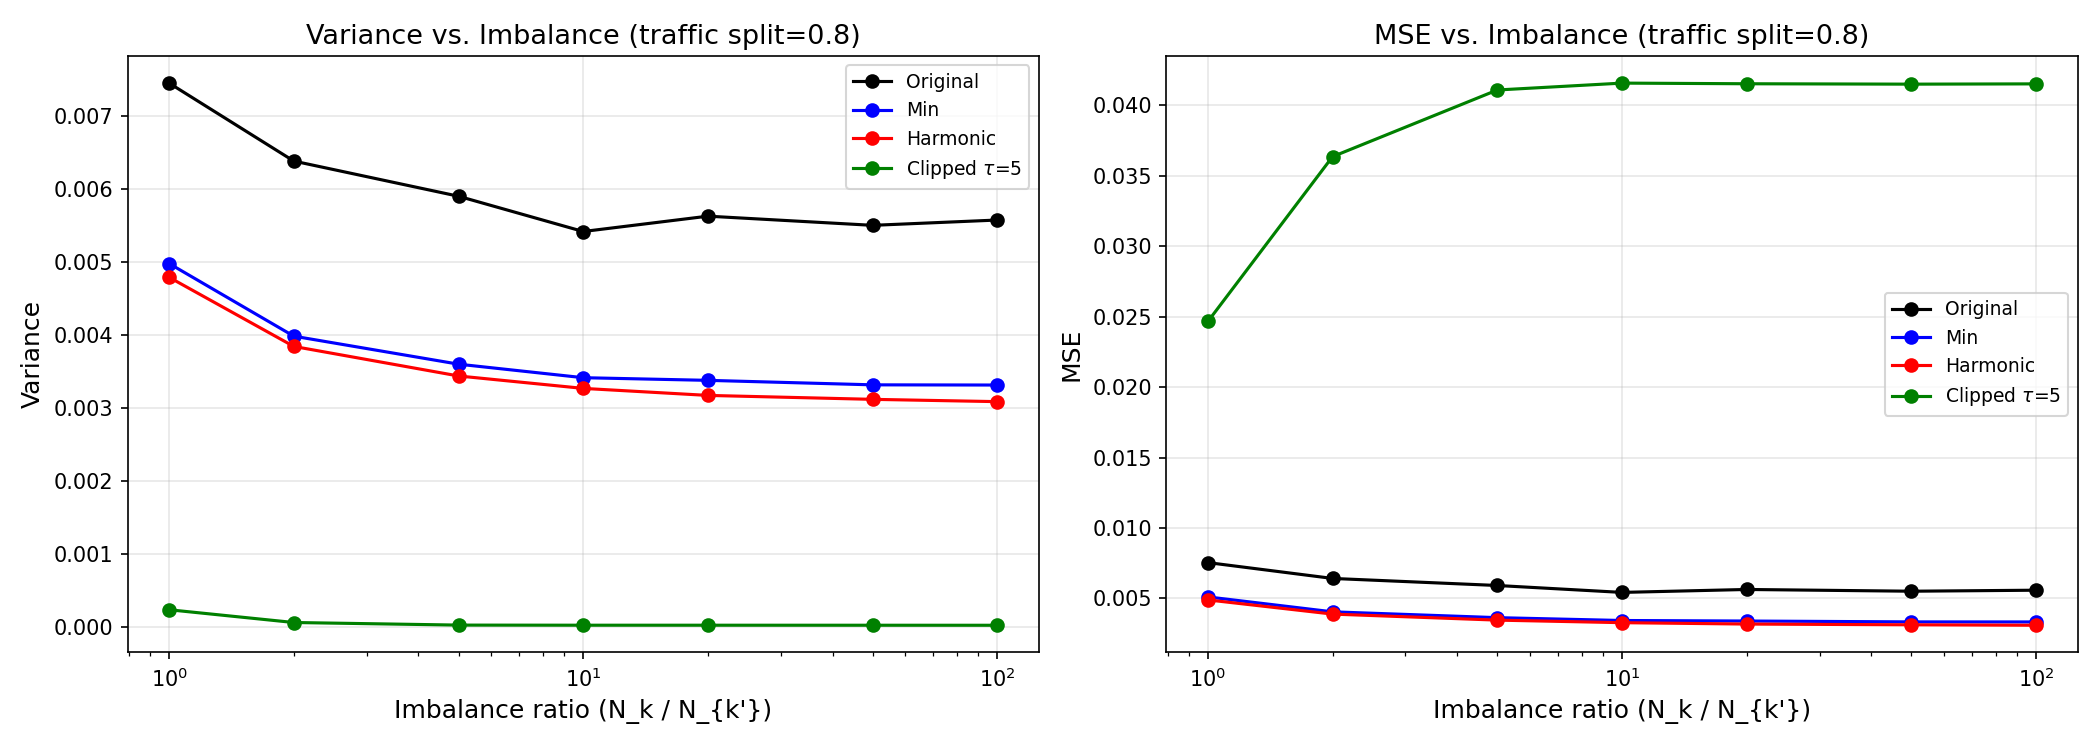
\includegraphics[width=0.48\textwidth]{../images/exp1_imbalance_sweep/exp1_variance_vs_imbalance.png}
    \caption{Variance vs.\ imbalance ratio at traffic split 80/20. Harmonic and min are consistently below original; clipped achieves near-zero variance at the cost of large bias$^2$ (see Table~\ref{tab:exp1_results}).}
    \label{fig:variance_vs_imbalance}
\end{figure}

\begin{table}[h]
    \small
    \centering
    \begin{tabular}{lcccc}
        \toprule
        Scheme & Var ($r=1$) & Var ($r=10$) & Var ($r=100$) & MSE ($r=100$) \\
        \midrule
        Original    & 0.00762 & 0.00593 & 0.00505 & 0.00507 \\
        Min         & 0.00521 & 0.00385 & 0.00300 & 0.00302 \\
        Harmonic    & 0.00513 & 0.00364 & 0.00285 & 0.00285 \\
        Clipped$_5$ & 0.00026 & 0.000024 & 0.000024 & 0.04151 \\
        \bottomrule
    \end{tabular}
    \caption{Variance and MSE at traffic split 80/20. Harmonic consistently outperforms both original and min. Clipped achieves near-zero variance but bias$^2 \approx 0.041$, giving MSE $\approx145\times$ higher than harmonic.}
    \label{tab:exp1_results}
\end{table}

Figure~\ref{fig:variance_reduction} shows variance reduction relative to original across all splits and ratios. At split $s=0.80$, ratio $r=100$, harmonic reduces variance by \textbf{43.6\%} versus original and by 5\% versus min. Crucially, harmonic never hurts: even at ratio $r=1$ (no systematic imbalance), it reduces variance by \textbf{32.7\%} because per-document count heterogeneity across queries remains—harmonic down-weights low-count documents, a benefit the uniform original weighting misses entirely. Reduction increases with traffic split, reaching \textbf{54\%} at $s=0.90$, $r=50$. Figure~\ref{fig:variance_vs_split} further shows this trend across all splits. The harmonic–min gap is consistent but modest ($\sim$5--7\%), reflecting that both schemes efficiently downweight the majority position when imbalance is severe; the advantage of harmonic lies in its principled optimality guarantee (Theorem~\ref{thm:optimality}) rather than a large empirical margin over min.

\begin{figure}[t!]
    \centering
    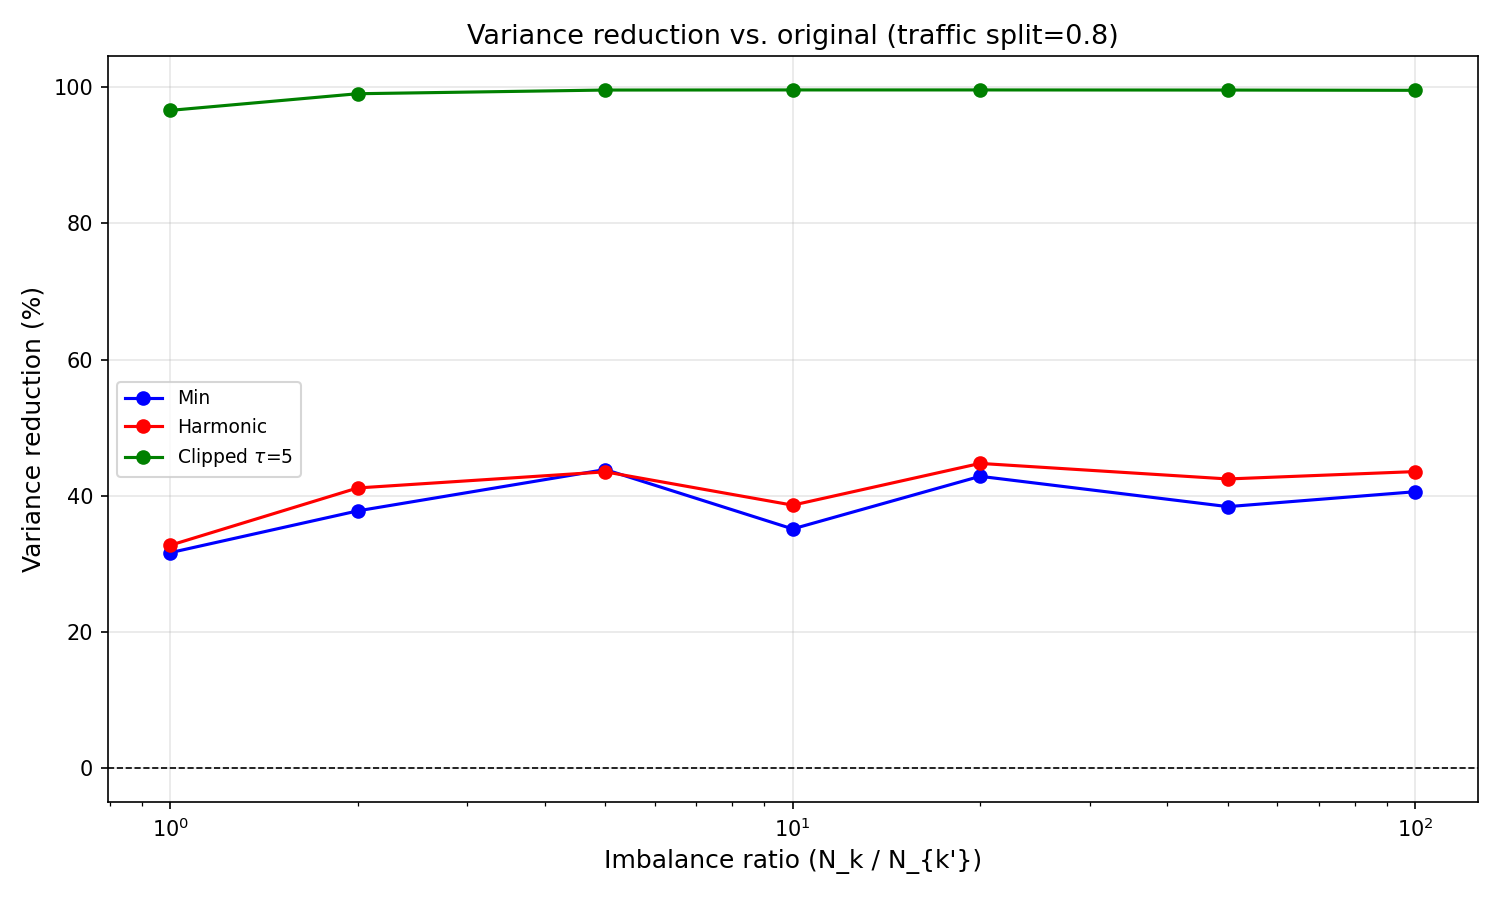
\includegraphics[width=0.48\textwidth]{../images/exp1_imbalance_sweep/exp1_variance_reduction.png}
    \caption{Variance reduction (\%) of harmonic and min relative to original, across traffic splits and imbalance ratios. Harmonic consistently dominates min; gains increase with both split and ratio.}
    \label{fig:variance_reduction}
\end{figure}

\begin{figure}[t!]
    \centering
    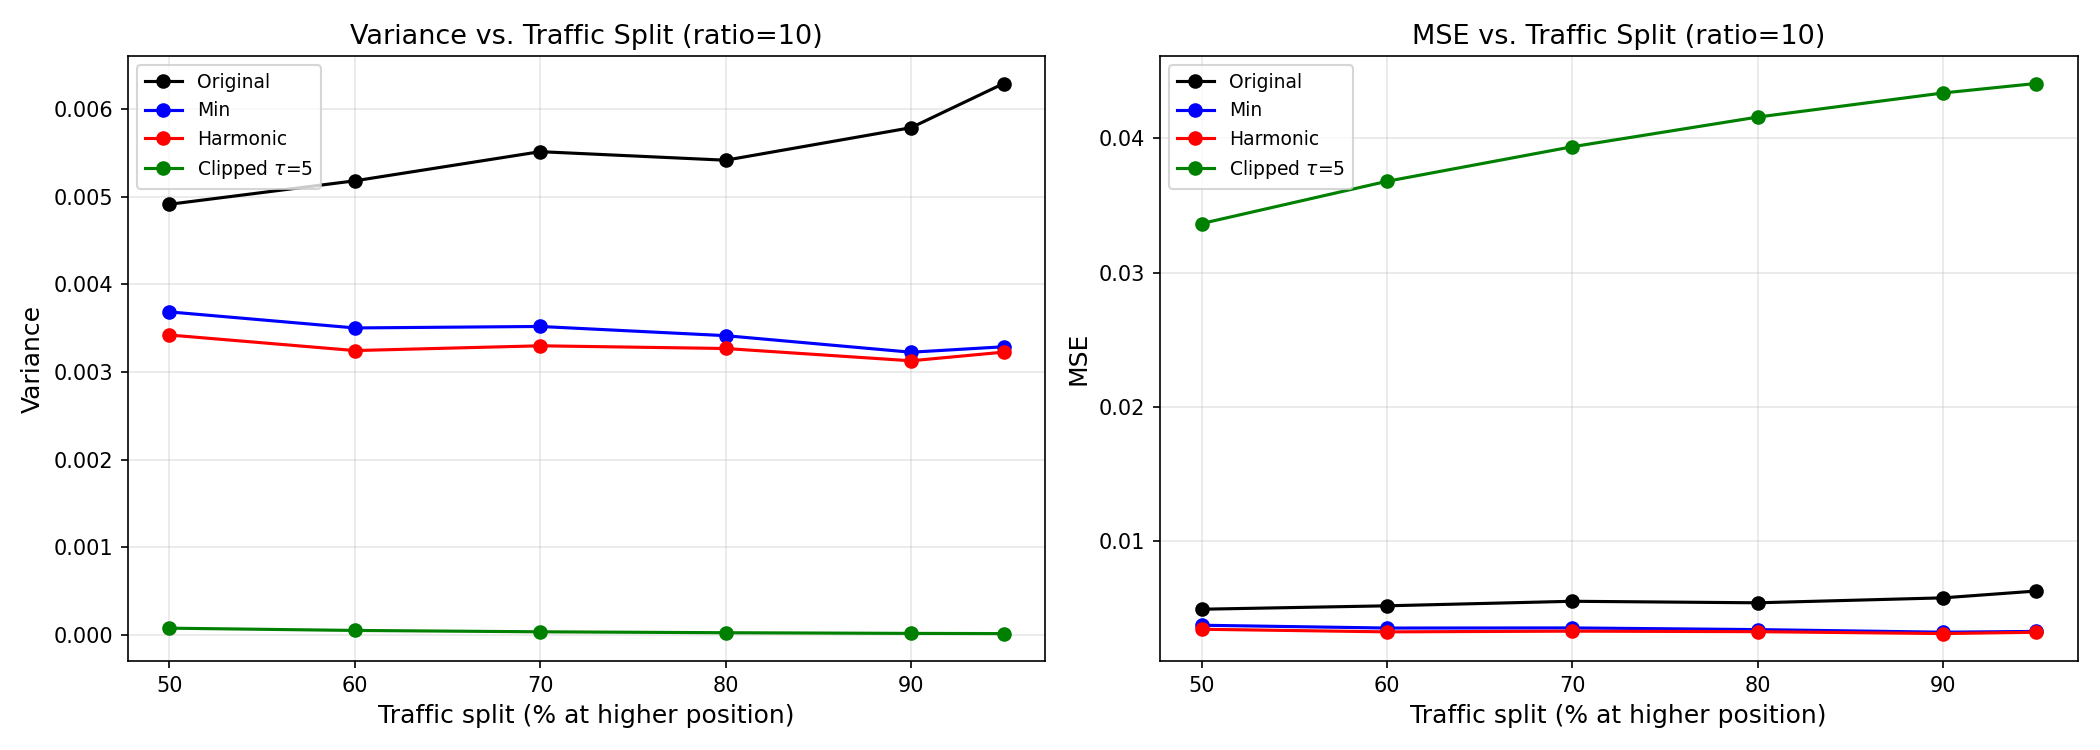
\includegraphics[width=0.48\textwidth]{../images/exp1_imbalance_sweep/exp1_variance_vs_split.png}
    \caption{Variance vs.\ traffic split at imbalance ratio 50:1. Harmonic and min consistently outperform original across all splits; gains grow as more documents become anchor items.}
    \label{fig:variance_vs_split}
\end{figure}

\subsection{Results: PBM Violations}

\begin{figure}[t!]
    \centering
    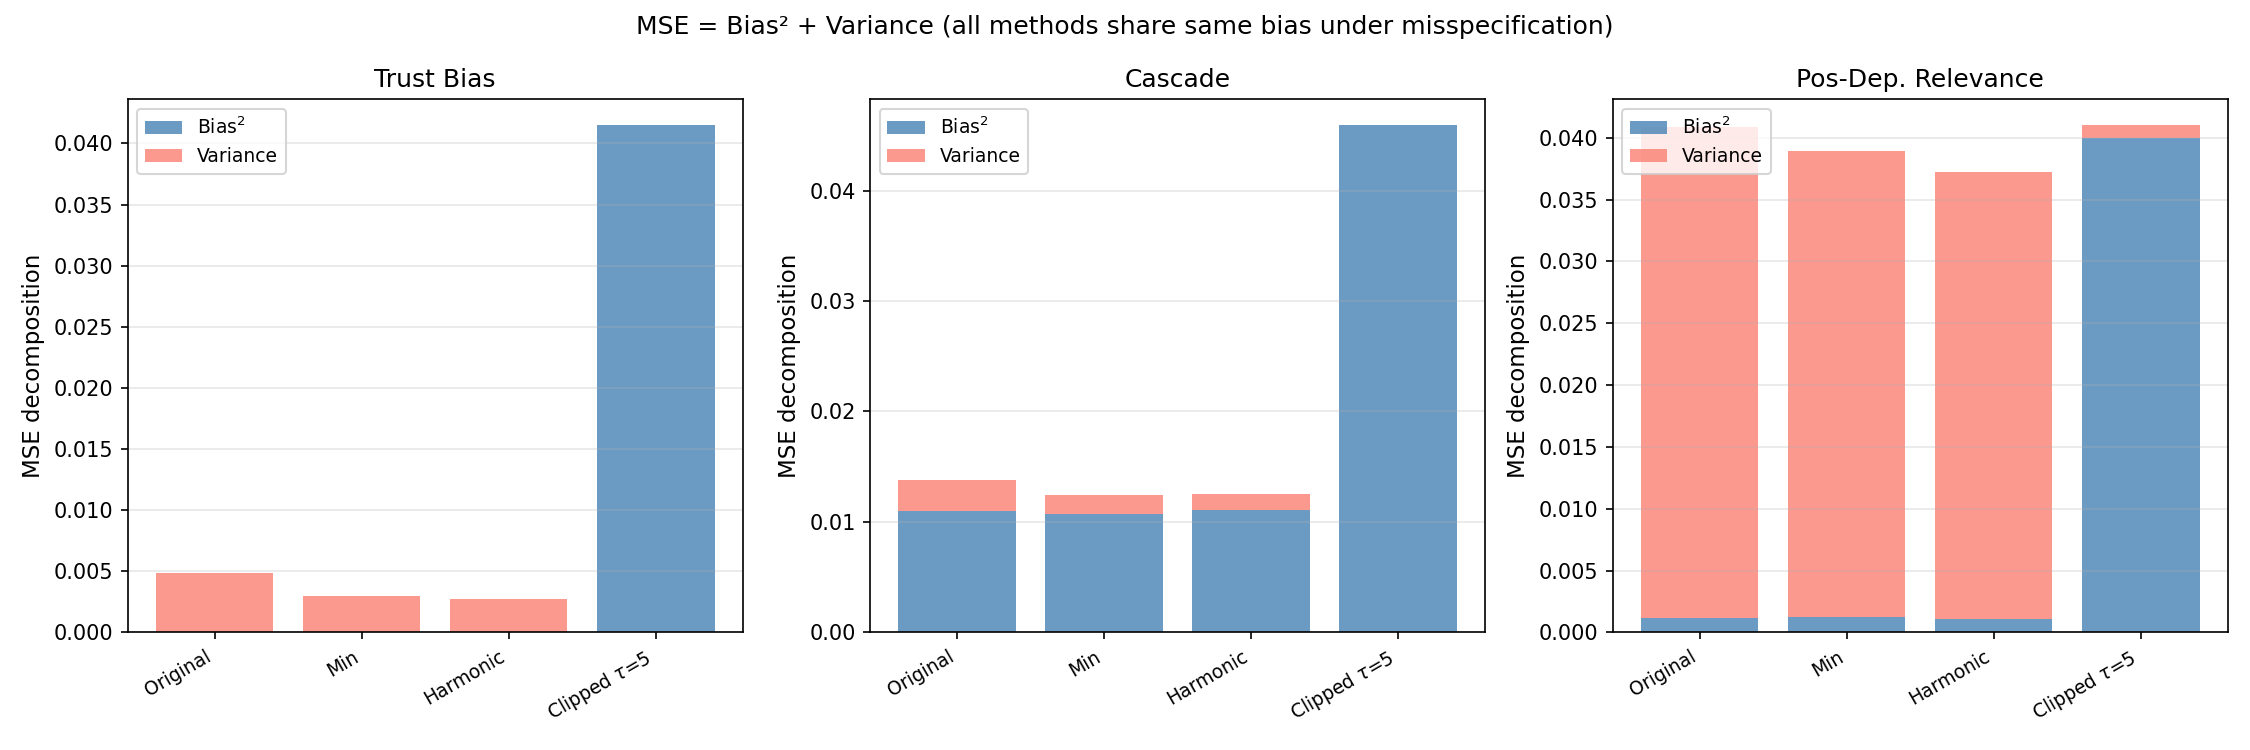
\includegraphics[width=0.48\textwidth]{../images/exp2_pbm_violations/exp2_mse_decomposition.png}
    \caption{MSE decomposition (bias$^2$ + variance) under two PBM violation models. Original, min, and harmonic share comparable bias$^2$ under both violations; harmonic achieves lower variance and thus lower MSE. Clipped weights introduce large additional bias.}
    \label{fig:pbm_violations}
\end{figure}

Figure~\ref{fig:pbm_violations} and Table~\ref{tab:pbm_violations} summarize results. Two findings stand out. First, original, min, and harmonic weighting all have \emph{comparable bias$^2$} under each violation model, substantially lower than clipped. This is consistent with all three being ratio-unbiased under PBM: when PBM fails, the residual bias within the intervention-harvesting family is determined by the model mismatch rather than the weight choice. Second, because bias is comparable across these three schemes, the lower variance of harmonic directly translates into lower MSE: 47\% lower than original under trust bias, 22\% lower under position-dependent relevance.

\begin{table}[h]
    \small
    \centering
    \begin{tabular}{llccc}
        \toprule
        Model & Scheme & MSE & Variance & Bias$^2$ \\
        \midrule
        \multirow{3}{*}{Trust}     & Original    & 0.00486 & 0.00485 & 7.5e-6 \\
                                    & Harmonic    & 0.00259 & 0.00259 & 2.7e-6 \\
                                    & Clipped$_5$ & 0.04152 & 2.0e-5  & 0.04150 \\
        \addlinespace
        \multirow{3}{*}{Pos.-dep.} & Original    & 0.03442 & 0.03335 & 0.00107 \\
                                    & Harmonic    & 0.02684 & 0.02592 & 0.00092 \\
                                    & Clipped$_5$ & 0.04090 & 7.5e-4  & 0.04015 \\
        \bottomrule
    \end{tabular}
    \caption{MSE decomposition under two PBM violations (anchor-item imbalance, split 80/20, ratio 50:1). Original and harmonic have comparable bias$^2$---far below clipped---while harmonic achieves 47\% lower variance under trust bias and 22\% lower under position-dependent relevance. Clipped's near-zero variance comes at the cost of $160\times$ higher bias$^2$.}
    \label{tab:pbm_violations}
\end{table}

\subsection{Experiment 4: Sample Efficiency}
\label{sec:exp4}

\begin{figure}[t!]
    \centering
    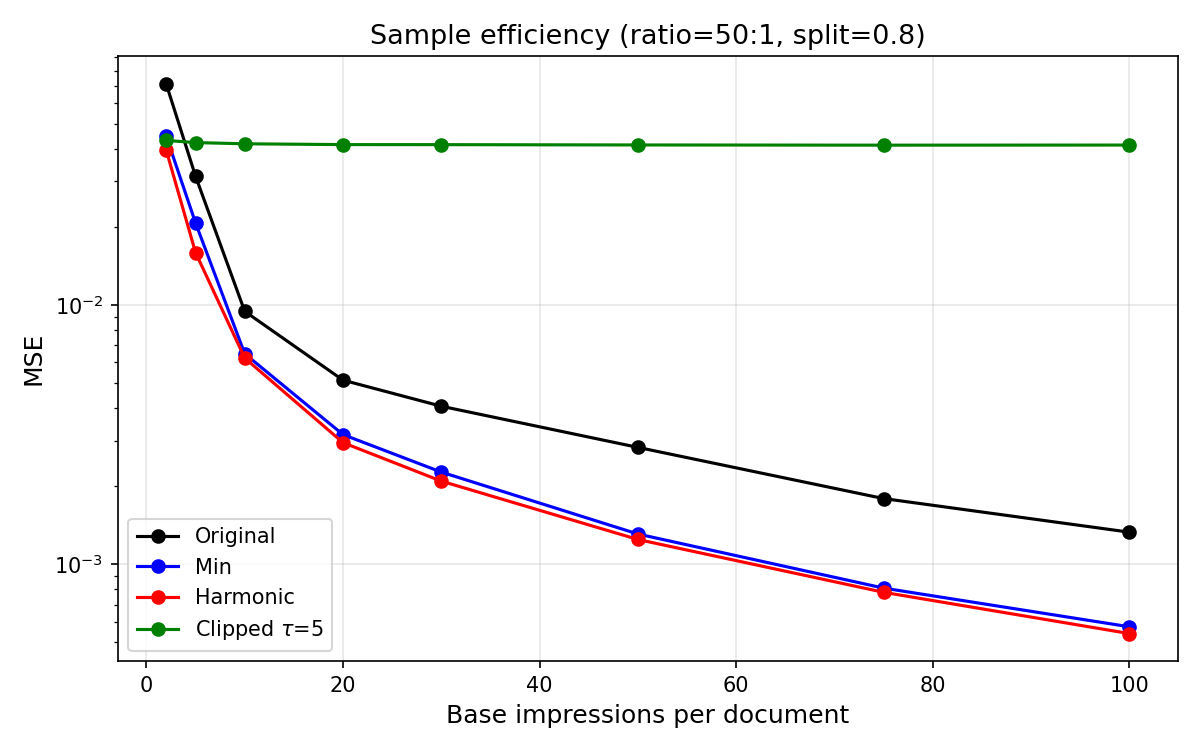
\includegraphics[width=0.46\textwidth]{../images/exp4_sample_efficiency/exp4_mse_vs_impressions.png}
    \caption{MSE vs.\ data volume (base impressions per document) at imbalance ratio 50:1, split 80/20. Harmonic reaches the same MSE as original with roughly half the data. Clipped's MSE is flat (bias-dominated) regardless of data volume.}
    \label{fig:sample_efficiency}
\end{figure}

A key practical claim is that lower variance translates directly to lower data requirements.
Figure~\ref{fig:sample_efficiency} sweeps data volume (base impressions per document, $b \in [2, 100]$) at fixed imbalance ratio 50:1 and traffic split 80/20.
MSE decreases monotonically for unbiased methods.
At $b=5$, harmonic achieves the same MSE as original at $b \approx 10$—a \textbf{2$\times$ data reduction} to reach equivalent accuracy.
At higher data volume the relative gap widens: at $b=50$, harmonic reduces MSE by \textbf{55.8\%}.
Clipped weighting's MSE is flat ($\approx 0.041$) regardless of data volume, confirming that its error is bias-dominated and no amount of additional data can correct it.

\subsection{Experiment 5: Variance Decomposition Verification}
\label{sec:exp5}

\begin{figure}[t!]
    \centering
    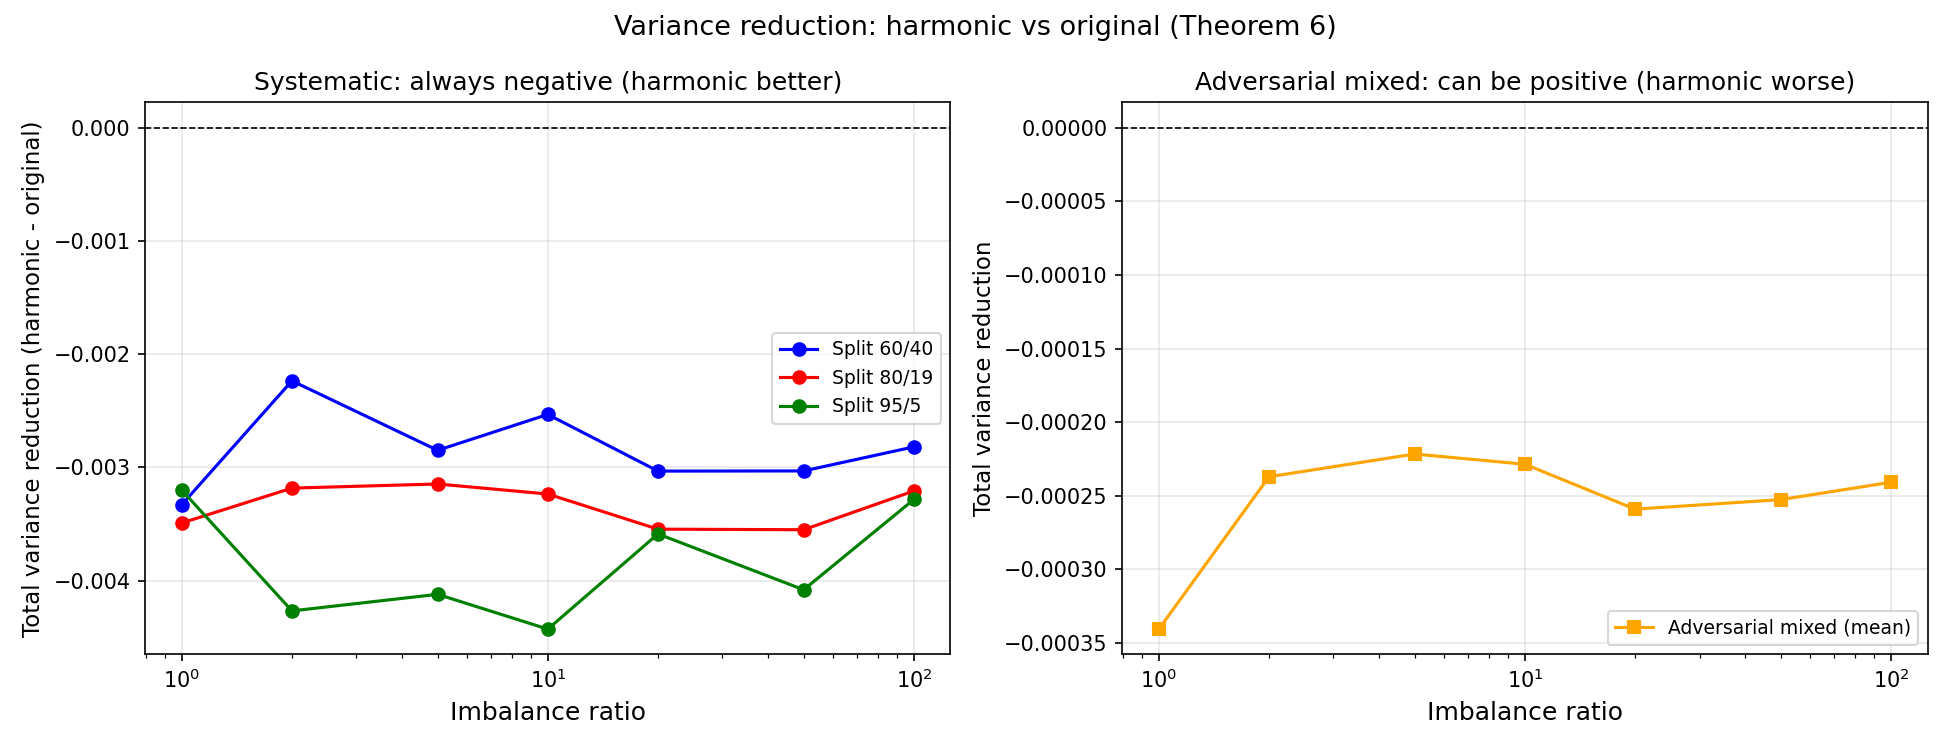
\includegraphics[width=0.48\textwidth]{../images/exp7_dk_condition/exp7_variance_reduction.png}
    \caption{Variance reduction achieved by harmonic vs.\ original across systematic and adversarial mixed-imbalance configurations. Harmonic reduces total variance in 100\% of systematic cases (Cauchy–Schwarz guarantee), and the $D_k \geq 0$ sufficient condition holds in 46.6\% of those cases.}
    \label{fig:dk_condition}
\end{figure}

We verify Theorem~\ref{thm:decomp} empirically across 189 systematic and 63 adversarial mixed-imbalance configurations (Figure~\ref{fig:dk_condition}). The Cauchy–Schwarz condition $D_k + D_{k'} \leq 0$ holds in 100\% of cases (0 violations), confirming Theorem~\ref{thm:cs}; total variance change $\alpha D_k + \beta D_{k'} \leq 0$ also holds in 100\% of systematic cases. The sufficient condition $D_k \geq 0$ holds in 46.6\% of cases, confirming it is not necessary.

\subsection{Experiment 3: Yahoo LTR Semi-Synthetic}
\label{sec:exp3}

To verify that results hold beyond uniform-random relevance, we repeat the imbalance sweep using \emph{real} relevance labels from the Yahoo Learning to Rank Challenge dataset (Set~1) \cite{chapelle2011yahoo}. We use the 6,936 test-set queries with graded relevance $g \in \{0,1,2,3,4\}$; continuous relevance is computed as $\mathrm{rel}(q,d) = (2^g - 1)/15$, following the standard NDCG formulation. Click probabilities follow PBM: $P(C=1|q,d,k) = p_k \cdot \mathrm{rel}(q,d)$. All other simulation parameters (anchor-item model, $M=10$, $\eta=1$, 200 trials) match Experiment~1.

\begin{table}[h]
    \small
    \centering
    \begin{tabular}{lcccc}
        \toprule
        Scheme & Var ($r=1$) & Var ($r=10$) & Var ($r=50$) & MSE ($r=50$) \\
        \midrule
        Original    & 0.00017 & 0.00015 & 0.00015 & 0.00015 \\
        Min         & 0.00011 & 0.00009 & 0.00009 & 0.00009 \\
        Harmonic    & 0.00010 & 0.00009 & 0.00009 & 0.00009 \\
        Clipped$_5$ & 0.00001 & 0.00000 & 0.00000 & 0.04120 \\
        \bottomrule
    \end{tabular}
    \caption{Variance and MSE on Yahoo semi-synthetic data (split 80/20). Harmonic consistently outperforms original and min. Clipped achieves near-zero variance but incurs large bias$^2$, giving MSE $\approx 458\times$ higher than harmonic at $r=50$.}
    \label{tab:yahoo_results}
\end{table}

\begin{figure}[t!]
    \centering
    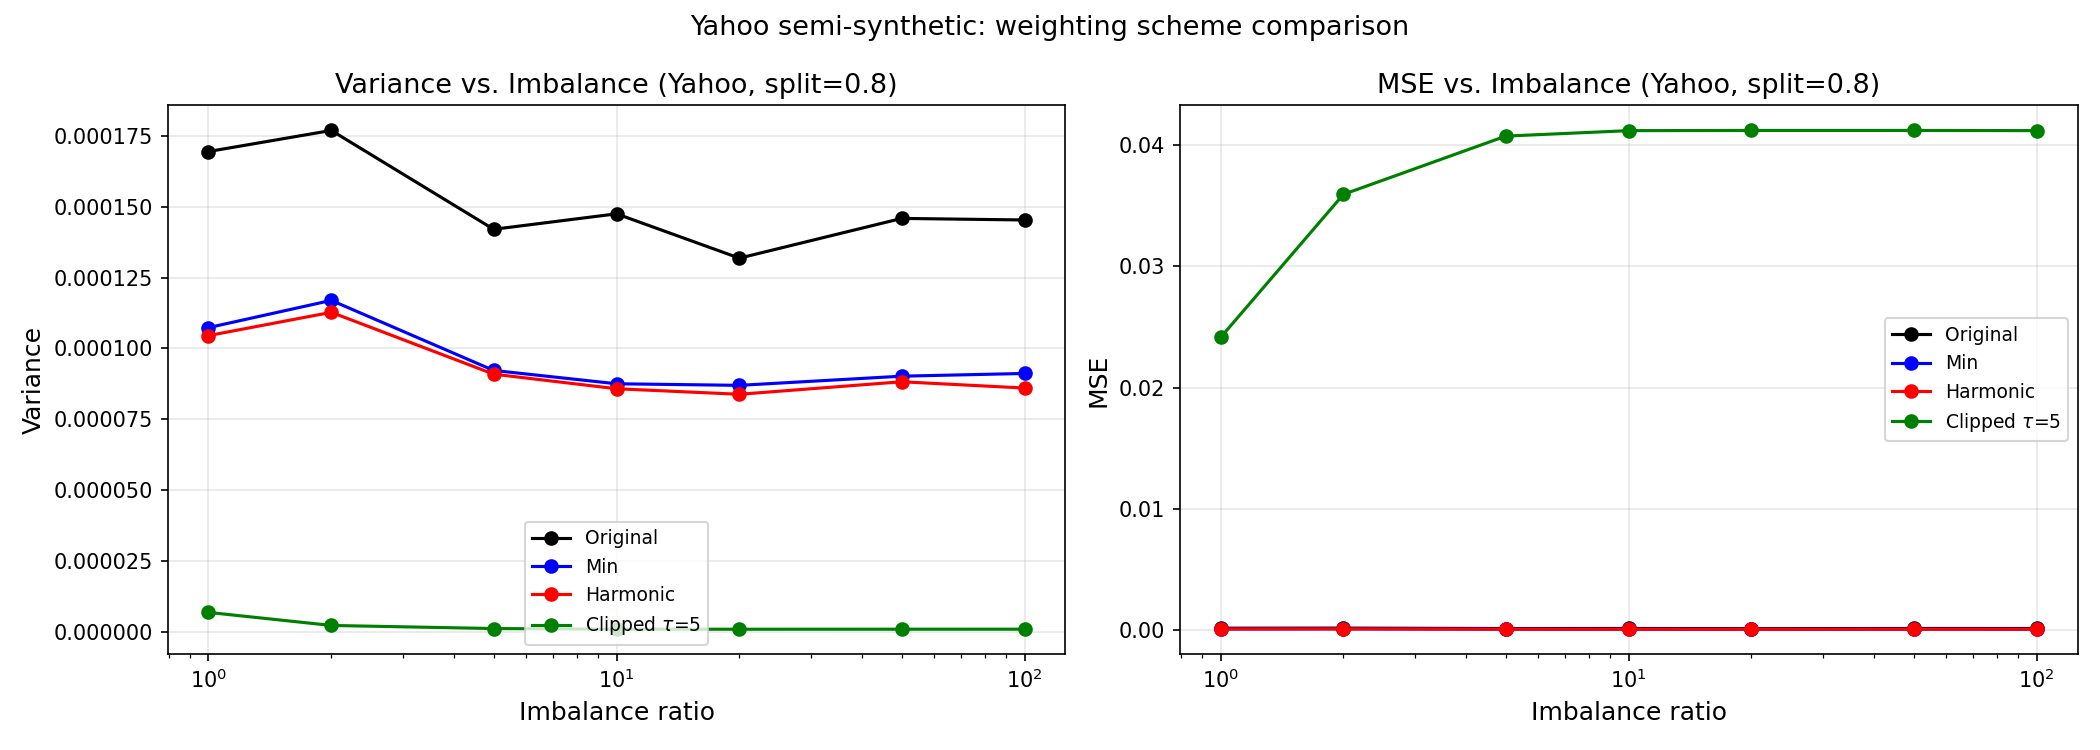
\includegraphics[width=0.48\textwidth]{../images/exp3_yahoo/exp3_variance_vs_imbalance.png}
    \caption{Variance and MSE vs.\ imbalance ratio on Yahoo semi-synthetic data (split 80/20). Harmonic consistently outperforms original and min across all ratios.}
    \label{fig:yahoo_variance}
\end{figure}

The results (Table~\ref{tab:yahoo_results} and Figure~\ref{fig:yahoo_variance}) confirm that harmonic weighting reduces variance by \textbf{39.5\%} versus original at ratio $r=50$, consistent with the fully synthetic results in Experiment~1 ($\sim$44\%). Harmonic reduces variance at every tested ratio, including $r=1$ (38.3\%), confirming no downside in the balanced regime. The relative ordering of all schemes is identical to the fully synthetic setting, confirming that variance reduction is driven by impression imbalance and not by the choice of relevance distribution.

\subsection{Experiment 6: Production A/B Testing Simulation}
\label{sec:exp6_prod}

A natural concern is whether anchor-item impression imbalance is realistic or synthetic. We simulate $K=5$ concurrent rankers: a default ranker (fraction $\alpha_0$ of traffic) shows each document at its natural position; treatment rankers independently swap adjacent pairs with probability 0.5. We compare uniform traffic (5$\times$20\%) against a production configuration (80\%\,+\,4$\times$5\%).

\begin{figure}[t!]
    \centering
    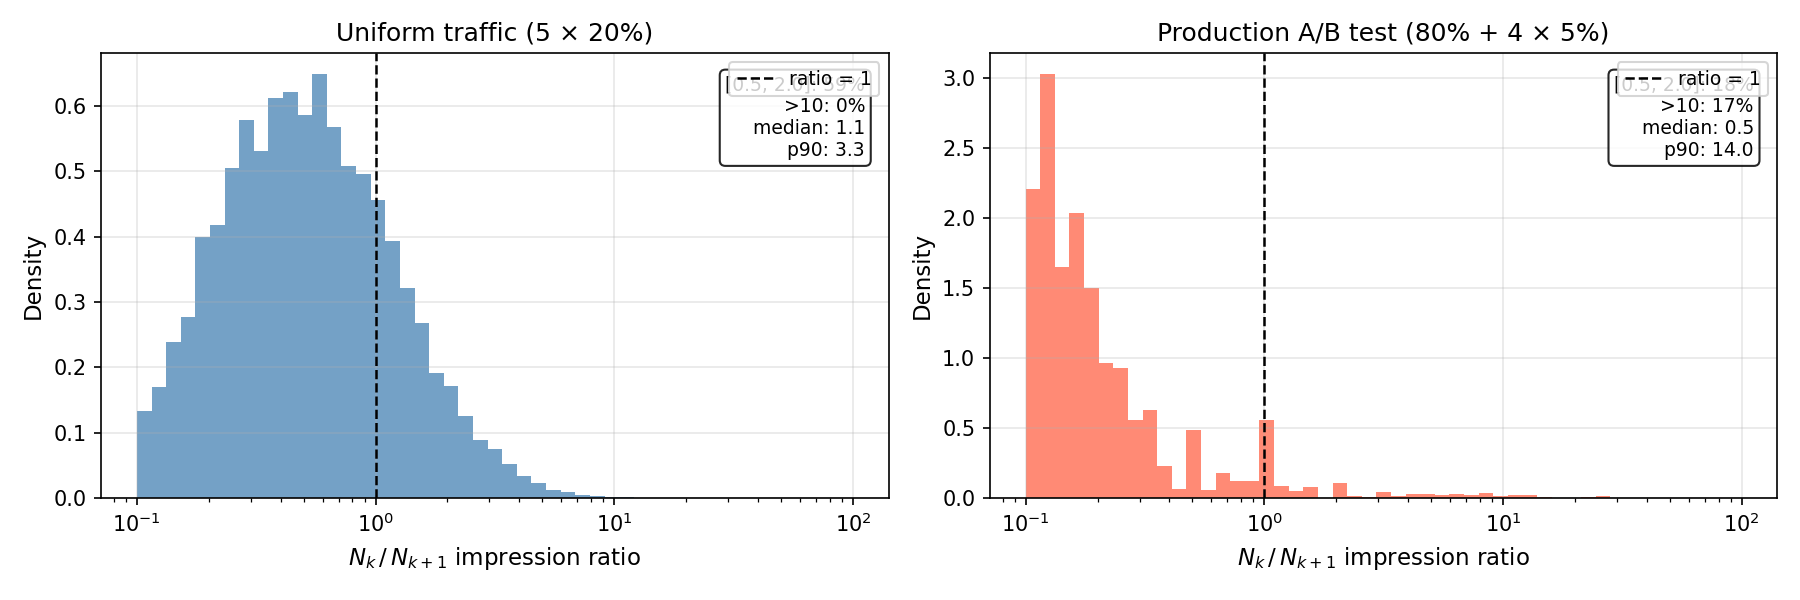
\includegraphics[width=0.48\textwidth]{../images/exp5_production/exp5_ratio_distribution.png}
    \caption{Impression ratio $N_k/N_{k+1}$ under uniform vs.\ production traffic. Production A/B testing creates a heavy-tailed distribution (16.7\% of pairs with ratio $>$10, p90$=$14); uniform traffic stays near ratio$=$1, consistent with Baidu-ULTR.}
    \label{fig:prod_ratio}
\end{figure}

Under uniform traffic, 58.9\% of adjacent pairs fall in $[0.5, 2.0]$ and only 0.4\% exceed~10---consistent with Baidu-ULTR (Section~\ref{sec:baidu}). Under the production configuration, only 18.5\% remain in $[0.5, 2.0]$ and 16.7\% exceed~10. Harmonic weighting reduces MSE by \textbf{17.2\%} in the production configuration vs.\ 6.3\% under uniform, confirming that the benefit scales directly with traffic-induced imbalance.

\subsection{Real-World Dataset: Absence of Impression Imbalance in Baidu-ULTR}
\label{sec:baidu}

A natural question is whether public benchmarks exhibit the impression imbalance that motivates our method.
We analysed the Baidu-ULTR dataset \cite{zou2022large} (train split, 14.5\,M rows, 12.3\,M unique $(q,d,\mathrm{pos})$ cells), which is the most widely used public click log for ULTR research.
We aggregated individual impressions to $(q, d, \mathrm{pos})$ cells and computed the following statistics:

\begin{itemize}
  \item \textbf{94.1\%} of $(q, d, \mathrm{pos})$ cells have $N = 1$ impression; \textbf{98.7\%} have $N \leq 3$ (mean 1.16).
  \item Only \textbf{4.3\%} of $(q, d)$ pairs appear at two or more distinct positions---the minimum requirement for any intervention harvesting estimator.
  \item Among the 454\,K adjacent-pair items that do qualify, the impression ratio $N_k / N_{k+1}$ is tightly concentrated near~1: \textbf{78.4\%} of pairs fall within $[0.5, 2.0]$, the median ratio is~1.0, and only 0.8\% exceed 10.
\end{itemize}

\noindent
These statistics confirm that Baidu-ULTR does not exhibit the systematic impression imbalance our method addresses.
Harmonic weighting offers no advantage over original in this regime: when $N_k \approx N_{k'}$, all $\omega_i^h = N_k N_{k'} / (N_k + N_{k'}) \approx N_k / 2$, and the ratio estimator reduces to the original.
The method is primarily relevant to production A/B-testing systems with proprietary logs where anchor documents accumulate disproportionate traffic at one position, as modelled in Experiments~\ref{sec:exp1}--\ref{sec:exp2}.

\section{Related Work and Conclusion}
\label{sec:related_work}

Position bias estimation methods broadly fall into three categories: randomized interventions, joint relevance-propensity models, and intervention harvesting.

\textbf{Randomized interventions} explicitly manipulate result rankings to estimate examination probabilities \cite{joachims2017unbiased, wang2018position}. These approaches guarantee unbiasedness by randomizing item placements, yet they significantly degrade the user experience due to intrusive changes in rankings \cite{Joachims2017}.

\textbf{Joint relevance-propensity models} simultaneously estimate relevance and propensity from observational data using techniques like Expectation-Maximization (EM) \cite{wang2018position, Wang2018}. Extensions such as PAL \cite{pai2020pal} integrate position-bias correction directly into CTR prediction models for recommender systems. While these methods are non-intrusive, they require a parametric relevance model; empirical comparison against intervention harvesting is therefore methodologically ill-posed, since the two paradigms solve different estimation problems (parametric relevance-and-propensity joint inference vs.\ model-free propensity-only estimation).

\textbf{Intervention harvesting approaches}, originally proposed by \cite{agarwal2019estimating}, leverage natural ranking variations from multiple historical rankers, eliminating explicit randomization. Such methods preserve user experience while producing unbiased propensity estimates without assuming a relevance model. Extensions of this idea include temporal fluctuations in e-commerce search rankings \cite{aslanyan2019eCommerceBias} and policy-aware estimation from bandit logs \cite{oosterhuis2023DoublyRobustLTR}.

Despite advances, propensity estimation remains prone to high variance with importance sampling \cite{swaminathan2015CRM}. Variance-reduction strategies include clipping \cite{bottou2013counterfactual}, self-normalized estimators \cite{swaminathan2015batch}, doubly robust estimators \cite{dudik2011doubly, oosterhuis2023DoublyRobustLTR}, and control variates \cite{kong1992note}. Doubly robust methods for LTR \cite{oosterhuis2023DoublyRobustLTR} target the ranking objective and are not directly comparable to model-free propensity estimation. Within the intervention harvesting family, applying SNIPS-style normalization to both $A$ and $B$ is a no-op: dividing both numerator and denominator by $\sum_i \omega_i$ leaves $\hat{R} = A/B$ unchanged; SNIPS targets absolute-quantity estimation, not ratios. Clipped weighting \cite{bottou2013counterfactual} is the natural biased low-variance reference included in our comparison.

Based on the intervention harvesting approach of \cite{agarwal2019estimating}, we proposed harmonic weighting for non-intrusive position bias estimation. Compared to the prior min-weighting heuristic \cite{agarwal2019estimating}, harmonic weighting has a principled theoretical foundation and consistent empirical advantages. Key contributions:
\begin{itemize}
  \item A unified ratio estimator framework: any count-dependent weight preserves ratio-unbiasedness (Theorem~\ref{thm:ratio_unbiased})
  \item An exact Cauchy–Schwarz guarantee: harmonic always reduces the variance surrogate $V_k + V_{k'}$ versus original weighting (Theorem~\ref{thm:cs}); via the delta-method approximation this implies lower $\mathrm{Var}(\hat{R}\mid\mathbf{N})$
  \item Harmonic is variance-optimal when $\alpha = \beta$ (Theorem~\ref{thm:optimality}), the dominant case for adjacent-position estimators; a decomposition theorem (Theorem~\ref{thm:decomp}) characterizes the asymmetric case
  \item Empirical validation showing up to 55\% variance reduction versus original, confirmed on Yahoo semi-synthetic and production A/B simulation; under tested PBM violations, original, min, and harmonic share comparable bias, making lower variance directly advantageous for MSE
\end{itemize}

Our implementation and all experiments presented in this paper will be publicly available after acceptance. The implementation builds upon the unbiased learning-to-rank toolkit by \cite{Hager2024}, which provides a comprehensive framework for position bias estimation and evaluation.

Several directions remain open. First, the Cauchy–Schwarz guarantee covers the per-pair ratio $\hat{R}_{k,k'}$; extending the variance analysis to the full AdjacentChain product estimator requires bounding error propagation through the chain. Second, the optimal weight $\omega_i^*$ depends on the unknown propensities; data-adaptive estimation of $\alpha/\beta$ from held-out data could close the remaining 2\% gap versus the oracle. Third, applying harmonic weighting to non-adjacent interventional sets (where $\alpha \neq \beta$ is more pronounced) and to doubly robust LTR objectives are natural extensions.



\bibliographystyle{ACM-Reference-Format}
\bibliography{refs}

\end{document}
